\documentclass[11pt, oneside]{article} 
\usepackage{geometry}
\geometry{letterpaper} 
\usepackage{graphicx}
	
\usepackage{amssymb}
\usepackage{amsmath}
\usepackage{parskip}
\usepackage{color}
\usepackage{hyperref}

\graphicspath{{/Users/telliott/Github/Tex/png/}}
% \begin{center} 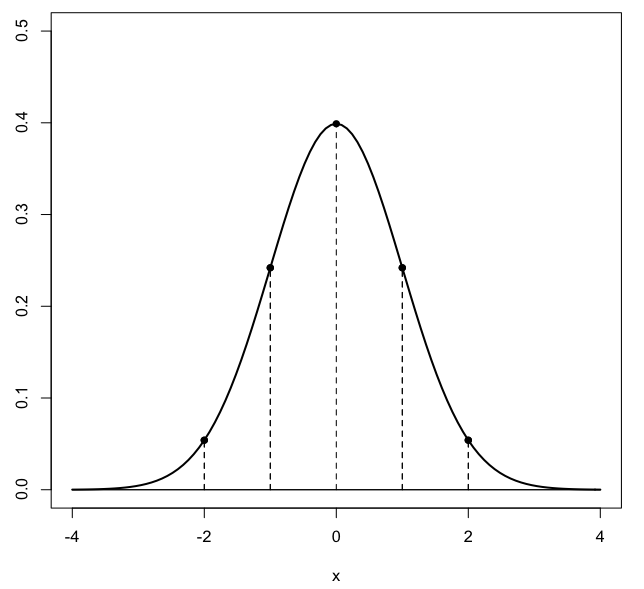
\includegraphics [scale=0.4] {gauss3.png} \end{center}

\title{Continuum of Numbers}
\date{}

\begin{document}
\maketitle
\Large

In a previous chapter we showed that given any two rational numbers one can find a rational number which lies between them.

Three related statements are also true.  We will show that

$\circ$ for any two rational numbers one can find a real number which lies between them

$\circ$ for any two real numbers one can find a rational number which lies between them

$\circ$ for any two real numbers one can find a real number which lies between them

\subsection*{continuum}

$\circ$  Between any two \emph{real} numbers it is always possible to find a rational number.  

Proof:  pick
\[ N \in \mathbb{N} \text{ such that } N > \frac{1}{b-a} \]
Then 
\[ \frac{1}{N} < b - a \]
Define the set $\mathbf{A}$ as follows:
\[ \mathbf{A} = \{ \ \frac{m}{N}: \ m \in \mathbb{N} \}, \ \ \ \text{a subset of } \mathbb{Q} \]
The claim is that
\[ \mathbf{A} \cap (a,b) \ne \emptyset \]
There do exist numbers within the open interval $(a,b)$ that are in the set $\mathbb{Q}$.

The proof is by contradiction.  Assume on the contrary that the set $\mathbf{A}$ does not contain a rational number lying inside this interval.  In other words:
\[ \mathbf{A} \cap (a,b) = \emptyset \]
Now, find the largest integer $m_1$ such that $m_1/N < a$ (it is OK if $m_1$ is equal to $0$).  Then the next rational number in $\mathbf{A}$ must be larger than $b$ since the set intersection is empty:
\[ \frac{m_1 + 1}{N} > b \]
But this implies that
\[ \frac{m_1 + 1}{N} - \frac{m_1}{N} > b - a \]
\[ \frac{1}{N} > b - a \]
which contradicts our condition on $N$ above.  Hence the assumption is false and so
\[ \mathbf{A} \cap (a,b) \ne \emptyset \]
Thus there must exist a rational number $r$ in $\mathbf{A}$ such that $a < r < b$.

\subsection*{example}
Consider the open interval:  $(\sqrt{2},\sqrt{3})$.  
\[ a = \sqrt{2} \approx 1.414 \]
\[ b = \sqrt{3} \approx 1.732 \]
\[ b-a \approx 0.3178 \]
\[ \frac{1}{b-a} \approx 3.1462 \]
Pick $N \ge 4$, for example
\[ N = 4: \ \ \  1.414 < \frac{6}{4} = 1.5 < 1.732 \]
\[ N = 5: \ \ \  1.414 < \frac{8}{5} = 1.6 < 1.732 \]
\[ N = 6: \ \ \  1.414 < \frac{9}{6} = 1.5 < 1.732 \]
(In this case $N=2$ and $N=3$ happen to work as well).

$\circ$  Between any two rational numbers it is always possible to find a real number.

One proof consists of finding a \emph{particular} irrational in the interval $(a,b)$, where $a$ and $b$ are rational.  For $a < b$, we simply add to the number $a$ the following
\[ c = \frac{\sqrt{2}}{2}(b - a) \]
$c$ is smaller than $b - a$ (because $\sqrt{2}/2 < 1$) so the result $a + c$ lies between $a$ and $b$.  We also know that $c$ is irrational, because $\sqrt{2}$ times any rational number is irrational.  Finally, $a + c$ is irrational because adding $\sqrt{2}$ times a rational number to any rational number produces an irrational number.

Proof of the first preliminary requirement:  $\sqrt{2}$ times a rational is irrational.  Suppose for integer $p, q, r, s$ we have
\[ \sqrt{2} \ \frac{p}{q} = \frac{r}{s} \]
then
\[ \sqrt{2} = \frac{rq}{ps} \]
But the right-hand side is rational, so this is a contradiction.

For the second requirement, again by contradiction suppose
\[ \sqrt{2} \ \frac{p}{q} +  \frac{s}{t} = \frac{u}{v} \]
for integer $p, q, r, s, u, v$.  But the right-hand side of
\[ \sqrt{2} = \frac{q}{p} ( \frac{u}{v} - \frac{s}{t}) \]
is rational, so this is a contradiction.

Note in passing that powers are different.  What do you think about
\[ r = \sqrt{2}^{\sqrt{2}} \]
You may think $r$ is "likely" to be irrational.  Just a mess.  But how about
\[ r^{\sqrt{2}} \]
Whether $r$ is rational or irrational
\[ r^{\sqrt{2}} = (\sqrt{2}^{\sqrt{2}})^{\sqrt{2}} = \sqrt{2}^2 = 2 \]
!!

$\circ$  Between any two real numbers it is always possible to find another real number.  This one is subtle.  Suppose the two real numbers are "really, really close."  

We suppose that they are not equal, so they must be different, say $a < b$.

Since they are different, at some stage in the decimal expansions of $a$ and $b$, there must be a first position at which $a$ and $b$ differ.  If $b$ does not have a $0$ at the next position, terminate there and that will be $c$.

For example:
\[ a = 1.23456789129.. \]
\[ b = 1.23456789133.. \]
\[ c = 1.23456789130.. \]

$b$ must have some digit following this first position where it does not match $a$, and which is also not equal to zero (otherwise it would be a terminating decimal and thus a rational number).  So we can always find a place to terminate to form $c$.

\textbf{Eternity is a very long time, especially towards the end. }

(credited to Woody Allen)

\subsection*{variations of infinity}
In other words there is \emph{no least number} $x$ such that $x > 0$, for example, and no greatest number $x$ such that $x < 1$.  

Proof:  Assume that $m$ is the smallest number $> 0$.  The rational number $m/2 < m$ is also greater than zero, but smaller than $m$.  Thus, $m$ is not the smallest positive number.

In general, there is no number that is the closest number to another number.

That is actually OK.  Here's what's really weird.  Cantor proved that the set $\mathbb{Q}$ is \emph{countably finite}.  Each element in $\mathbb{Q}$ can be paired in order with a member of $\mathbb{N}$.

The idea of the proof is to show that one can set up a correspondence between $\mathbb{N}$ and $\mathbb{Q}$, assigning each number $r \in \mathbb{Q}$ in a particular order to $1,2,3, \dots$.  Here is the figure from Courant and John:
\begin{center} 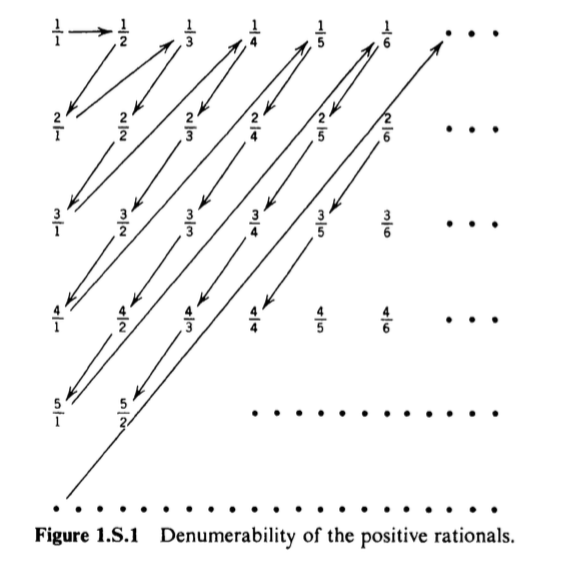
\includegraphics [scale=0.5] {denumerability.png} \end{center}
Basically, each row contains all the rational numbers with a particular numerator, and each column contains all the numbers with a particular denominator, arranged in strict increasing order.

Next, set up the sequence indicated by the arrows:
\[ \frac{1}{1} \ \ \ \ \ \frac{1}{2}, \frac{2}{1} \ \ \ \ \  \frac{1}{3}, \frac{2}{2}, \frac{3}{1} \ \ \ \ \ \frac{1}{4}, \frac{2}{3}, \frac{3}{2}, \frac{4}{1} \ \ \ \ \ \frac{1}{5}, \frac{2}{4}, \frac{3}{3}, \frac{4}{2}, \frac{5}{1} \ \ \ \ \ \frac{1}{6}, \frac{2}{5}, \frac{3}{4}, \frac{4}{3}, \frac{5}{2}, \frac{6}{1} \dots \]
Then remove all fractions that are duplicates because they are not in lowest terms.
\[ \frac{1}{1} \ \ \ \ \ \frac{1}{2}, \frac{2}{1} \ \ \ \ \  \frac{1}{3}, \frac{3}{1}\ \ \ \ \ \frac{1}{4}, \frac{2}{3}, \frac{3}{2}, \frac{4}{1} \ \ \ \ \ \frac{1}{5}, \frac{5}{1} \ \ \ \ \  \frac{1}{6}, \frac{2}{5}, \frac{3}{4}, \frac{4}{3}, \frac{5}{2}, \frac{6}{1} \dots \]

Finally, each $r$ in this sequence is assigned to a natural number (in the sequence $\mathbb{N}$), establishing the denumerability property.  $1/3$ is paired with $4$ and $3/1$ is paired with $5$, and so on.

Cantor showed that such a correspondence (which we just established for $\mathbb{Q}$), is impossible for $\mathbb{R}$.  The proof of this is not hard, but we will skip it here.  You can check out the chapters on Georg Cantor in Dunham's \emph{Journey Through Genius}.

Thus, the rational numbers are said to be "countably infinite", while the real numbers are not countable.  (There is also a proof that the transcendental numbers are much more numerous than the non-transcendental ones).

We say that the set of numbers greater than $0$ has \emph{no least element}.  We can test this by picking the smallest rational member imaginable, but subsequently, we can always find a smaller rational element (say, by halving that number).  

And once we get really close with the small rational element, there are infinitely more irrational than rational ones waiting beyond.  And yet, given any such very close irrational number, we can always find a smaller rational number, still larger than the bound.

I told you it was weird.

This property of the real numbers, that there is no closest number to any given number, accounts for virtually all of the theoretical difficulties in calculus which are solved by the use of limits and the apparatus of $\delta$ and $\epsilon$ or alternatively, neighborhoods.  We will get to that in a bit.

\end{document}